\documentclass[12pt]{article}

\usepackage{amsmath, mathtools}
\usepackage{amsfonts}
\usepackage{amssymb}
\usepackage{graphicx}
\usepackage{caption}
\usepackage{colortbl}
\usepackage{xr}
\usepackage{hyperref}
\usepackage{longtable}
\usepackage{xfrac}
\usepackage{tabularx}
\usepackage{float}
\usepackage{siunitx}
\usepackage{booktabs}
\usepackage{caption}
\usepackage{pdflscape}
\usepackage{afterpage}
\usepackage{cite}

\hypersetup{
    bookmarks=true,         % show bookmarks bar?
      colorlinks=true,       % false: boxed links; true: colored links
    linkcolor=red,          % color of internal links (change box color with linkbordercolor)
    citecolor=green,        % color of links to bibliography
    filecolor=magenta,      % color of file links
    urlcolor=cyan           % color of external links
}

%% Comments

\usepackage{color}

\newif\ifcomments\commentstrue %displays comments
%\newif\ifcomments\commentsfalse %so that comments do not display

\ifcomments
\newcommand{\authornote}[3]{\textcolor{#1}{[#3 ---#2]}}
\newcommand{\todo}[1]{\textcolor{red}{[TODO: #1]}}
\else
\newcommand{\authornote}[3]{}
\newcommand{\todo}[1]{}
\fi

\newcommand{\wss}[1]{\authornote{magenta}{SS}{#1}} 
\newcommand{\plt}[1]{\authornote{cyan}{TPLT}{#1}} %For explanation of the template
\newcommand{\an}[1]{\authornote{cyan}{Author}{#1}}

%% Common Parts

\newcommand{\progname}{Software Engineering} 
\newcommand{\authname}{Team \#6, Six Sense
\\ Omar Alam
\\ Sathurshan Arulmohan
\\ Nirmal Chaudhari
\\ Kalp Shah
\\ Jay Sharma
}        

\usepackage{hyperref}
    \hypersetup{colorlinks=true, linkcolor=blue, citecolor=blue, filecolor=blue,
                urlcolor=blue, unicode=false}
    \urlstyle{same}
                                


% For easy change of table widths
\newcommand{\colZwidth}{1.0\textwidth}
\newcommand{\colAwidth}{0.13\textwidth}
\newcommand{\colBwidth}{0.82\textwidth}
\newcommand{\colCwidth}{0.1\textwidth}
\newcommand{\colDwidth}{0.05\textwidth}
\newcommand{\colEwidth}{0.8\textwidth}
\newcommand{\colFwidth}{0.17\textwidth}
\newcommand{\colGwidth}{0.5\textwidth}
\newcommand{\colHwidth}{0.28\textwidth}

% Numbering 
\usepackage{amsthm}
\usepackage{xassoccnt}
%\newtheorem{req}{Requirement}[section]        
\newtheorem{req}{Requirement}        
\theoremstyle{definition}        
\newtheorem{constraint}{Constraint}
\newtheorem{goal}{Goal}
\DeclareCoupledCountersGroup{theorems}
\DeclareCoupledCounters[name=theorems]{req,constraint,goal}
\setcounter{goal}{0}

\usepackage{fullpage}

\setlength{\parindent}{0pt} % Set no indent to entire document.

\begin{document}

\title{Software Requirements Specification for \progname} 
\author{\authname}
\date{\today}
	
\maketitle

~\newpage

\pagenumbering{roman}

\tableofcontents

~\newpage

\section*{Revision History}


\begin{tabularx}{\textwidth}{p{3cm}p{2cm}X}
\toprule {\bf Date} & {\bf Version} & {\bf Notes}\\
\midrule
2025-10-06 & 1.0 & Initial Write-up\\
\bottomrule
\end{tabularx}


~\newpage

\pagenumbering{arabic}

\section{Goal}

\subsection{G.1 Context and overall objective}

With around 4 million Canadians affected by hearing loss \cite{Healthing2025}, 
there is a significant need for assistive technologies that can improve 
situational awareness and safety.
Many safety cues and general sound alerts such as the sound of a car 
approaching, a kettle whistling,
or a phone ringing may be missed, leading to increased risk of injury and
miscommunication.

Many existing solutions focus on speech transcription, but lack the ability to
provide directional information about sound sources or classify non-speech
sounds. This project aims to address this gap by developing an assistive device
that provides real-time visual indications of sound source locations and 
classifications.

The objective of this project is to develop an assistive device that aids
individuals who are deaf or hard of hearing by providing real-time visual
indications of sound source locations and classifications (ex. 'car on your 
left').

Some of the high-level goals of the project are:

\begin{goal}\label{goal:audio_capture}
Capture real-time audio data from a 
\hyperref[def:microphone_array]{microphone array}
with synchronized sampling to enable accurate situational analysis
of sound sources.
\end{goal}

\begin{goal}\label{goal:audio_direction_analysis}
Analyze captured audio to determine the direction of arrival (DoA) of
sound sources with minimal error and with minimal latency nearing real-time.
\end{goal}

\begin{goal}\label{goal:audio_identification_analysis}
Analyze captured audio to classify the sound sources with their English
label (ex. 'car', 'phone', 'kettle', 'alarm', 'speech').
\end{goal}

\begin{goal}\label{goal:visual_display}
Display audio classification and transcription on smart glasses in real-time
without obstructing the user's field of view.
\end{goal}

\begin{goal}\label{goal:user_friendly_interaction}
Provide a user-friendly interaction with the smart glasses,
allowing the user to easily set up, use, and understand visual indicators.
\end{goal}

\begin{goal}\label{goal:user_comfort}
Ensure that the system is comfortable to wear for extended periods of time,
with minimal discomfort or fatigue.
\end{goal}
    
\subsection{G.2 Current situation}

Currently, individuals who are deaf or hard of hearing face significant
challenges in maintaining situational awareness due to missed audio cues.
Existing assistive technologies address some aspects of this problem, but
leave critical gaps:

\begin{itemize}
\item \textbf{Smart glasses with transcription capabilities:} Some devices
can listen to live human audio and transcribe it to text (multilingual) in
real-time, displaying the transcript on a smartphone display.
However, these solutions focus solely on speech transcription and do not
provide directional information about sound sources or classify non-speech
sounds.

\item \textbf{Hearing aids:} Traditional hearing aids amplify ambient sounds
to improve awareness of audio sources at various volumes \cite{NIDCD2022}. 
While this helps individuals with partial hearing loss, it does not assist 
those who are profoundly deaf, nor does it provide visual cues about sound 
direction or classification.

\item \textbf{Notification systems:} Some home automation systems can send
visual alerts (e.g., flashing lights) when specific sounds are detected,
such as doorbells or smoke alarms. However, these systems are limited to
fixed locations and predetermined sound types, lacking portability and
real-time directional awareness.
\end{itemize}

The current solutions fail to address the critical need for real-time,
portable, directional awareness of environmental sounds, leaving individuals
vulnerable to missing important safety cues such as approaching vehicles,
warning beeps from machinery, or emergency alerts.

\subsection{G.3 Expected benefits}

The proposed system will deliver significant improvements to the daily lives
and safety of individuals who are deaf or hard of hearing:

\begin{itemize}
\item \textbf{Real-time spatial awareness:} Enable identification of sound
source locations on a 2D plane in real-time, allowing users to quickly
orient themselves toward important sounds such as someone calling their name,
an approaching vehicle, or an emergency alarm.

\item \textbf{Enhanced safety:} Reduce the risk of injury by alerting users
to critical safety cues that are typically communicated through sound, such
as warning beeps from forklifts, tea kettles whistling, car engines
or emergency sirens (from emergency vehicles) approaching from behind.

\item \textbf{Improved situational awareness:} Provide continuous awareness
of the acoustic environment without requiring the user to constantly scan
their surroundings, reducing cognitive load and enabling more natural
interactions with their environment.

\item \textbf{Sound classification:} Differentiate between various types of
sounds (e.g., speech, alarms, vehicles, household appliances) to help users
prioritize their attention and responses appropriately.

\item \textbf{Reduced frustration and miscommunication:} Minimize instances
of missed phone calls, doorbell rings, or verbal attempts to gain the user's
attention, leading to smoother social interactions and reduced social
isolation.

\item \textbf{Portable and wearable solution:} Unlike fixed home automation
systems, the smart glasses form factor provides continuous protection and
awareness regardless of location, whether at home, work, or in public spaces.

\item \textbf{Independence and confidence:} Empower users to navigate their
environment more independently without relying on others to alert them to
important sounds, fostering greater autonomy in daily activities.
\end{itemize}



\subsection{G.4 Functionality overview}

The system will provide the following principal functions:

\begin{itemize}
\item \textbf{Real-time audio capture:} Continuously capture audio signals
from a synchronized microphone array mounted on smart glasses, ensuring
precise temporal alignment for accurate spatial analysis.

\item \textbf{Direction of arrival (DoA) estimation:} Process captured audio
to determine the angular direction of sound sources on a 2D plane relative
to the user's position, with a target accuracy of ±45° for single sound
sources.

\item \textbf{Sound source classification:} Analyze audio characteristics to
classify detected sounds into meaningful categories (e.g., speech, vehicle
sounds, alarms, household appliances) using audio fingerprinting techniques,
with a target accuracy of at least 90\%.

\item \textbf{Visual feedback generation:} Generate intuitive visual
representations of detected sound sources, including their direction and
classification, displayed on the smart glasses interface with minimal
latency ($\leq$1 second).

\item \textbf{Multi-source handling:} Detect and track multiple simultaneous
sound sources when feasible, prioritizing the most relevant or critical
sounds based on classification and proximity.

\item \textbf{Real-time processing:} Execute all signal processing,
direction estimation and classification algorithms real-time,
with consistent performance and low latency.

\item \textbf{Noise cancellation or audio filtering:} The system will
modify or filter the actual sounds in the environment based on direction
of arrival in order to improve directional hearing. This would help improve
the quality of the transcriptions provided by the system.
\end{itemize}

\subsection{G.5 High-level usage scenarios}

The following scenarios illustrate fundamental usage paths through the system:

\subsubsection{Scenario 1: Pedestrian crossing detection}
A user is walking in an urban environment and approaches a street
intersection. As they prepare to cross, a car approaches from their left
side. The system detects the engine sound, estimates its direction (e.g.,
90° to the left), classifies it as a vehicle, and displays a visual
indicator on the smart glasses showing the direction and classification.
The user recognizes the alert and waits for the vehicle to pass before
crossing safely.

\subsubsection{Scenario 2: Kitchen safety alert}
A user is cooking in their kitchen when a tea kettle on the stove begins
to whistle. The system captures the high-pitched sound through the
microphone array, determines that it is coming from behind and to the
right (e.g., 135°), classifies it as a kettle or alarm sound, and displays
a directional indicator. The user turns toward the alert and removes the
kettle from heat, preventing a potential hazard.

\subsubsection{Scenario 3: Social interaction}
A user is in a crowded room when someone calls their name from across the
space. The system detects the speech sound, estimates the direction (e.g.,
30° to the right), classifies it as speech or a human voice, and displays
the information on the glasses. The user turns in the indicated direction
to make eye contact and engage in conversation, reducing social friction
and missed interactions.

\subsubsection{Scenario 4: Workplace awareness}
A user is working in an industrial setting when a forklift begins reversing
nearby, emitting a warning beep. The system detects the beeping pattern,
determines its direction (e.g., directly behind at 180°), classifies it as
a warning signal, and alerts the user with a prominent visual indicator.
The user steps aside to maintain a safe distance from the moving equipment.

\subsection{G.6 Limitations and exclusions}

The following aspects are explicitly outside the scope of this project:

\begin{itemize}
\item \textbf{Autonomous danger assessment:} The system will not independently
evaluate whether a detected sound represents an immediate danger or
automatically alert the user of hazardous situations. It will present
directional and classification information, leaving interpretation and
response decisions to the user.

\item \textbf{Augmented reality overlay:} The system will not provide
full augmented reality capabilities with spatial overlays showing sound
locations directly mapped onto the user's field of view. Visual feedback
will be presented through a simpler display interface on the smart glasses.

\item \textbf{User response monitoring:} The system will not track whether
the user has noticed, acknowledged, or responded to presented alerts. There
is no feedback loop to ensure user reaction or to escalate notifications.

\item \textbf{Multilingual speech transcription:} Audio transcription
functionality, if implemented, will be limited to English only. Support
for other languages is not included in the current scope.

\item \textbf{3D spatial localization:} Direction estimation will be
constrained to a 2D horizontal plane around the user. Elevation angle
determination (above or below the user's head level) is excluded from
the core functionality.

\item \textbf{Sound source distance estimation:} While direction will be
provided, the system will not attempt to estimate the absolute distance
to sound sources.

\item \textbf{Continuous recording or data storage:} The system will not
record or store audio data beyond what is necessary for real-time processing.
No historical logs of detected sounds will be maintained.

\item \textbf{Network connectivity:} All processing will
occur locally on the embedded hardware. The system will not require internet
connectivity or cloud-based services for core functionality.
\end{itemize}

\subsection{G.7 Stakeholders and requirements sources}

\subsubsection{Primary stakeholders}

\begin{itemize}
\item \textbf{Individuals who are deaf or hard of hearing:}
\label{stakeholder:hardHearing} The primary
end-users of the system, who will directly benefit from improved
situational awareness and safety. This group is quite large in population,
with approximately 4 million people who experience hearing loss 
in Canada alone (1 in 10). The McMaster Sign Language club is a group at
McMaster University that falls in this stakeholder group.

\end{itemize}

\subsubsection{Secondary stakeholders}

\begin{itemize}
\item \textbf{Family members and caregivers:} Individuals who support people
with hearing loss and will benefit from improved communication and reduced
safety concerns.

\item \textbf{Employers and workplace safety officers:} Organizations that
employ individuals with hearing loss and are responsible for maintaining
safe working environments.

\item \textbf{Accessibility advocates and organizations:} Groups focused on
improving quality of life and independence for individuals with disabilities.

\item \textbf{Healthcare providers and audiologists:} Professionals who may
recommend or integrate such assistive technologies into patient care plans.

\item \textbf{Future developers and researchers:} The broader engineering
and scientific community who may build upon this work or apply similar
techniques to related problems.
\end{itemize}

\subsubsection{Requirements sources}

\begin{itemize}
\item \textbf{Academic literature:} Research on hearing loss impact,
assistive technologies, direction of arrival algorithms, and audio
classification techniques.

\item \textbf{Domain experts:}\label{itm:domain-experts} Consultation with domain experts, such as 
Dr. Mohrenschildt, for technical feasibility and requirements validation.

\item \textbf{Existing assistive technologies:} Analysis of current solutions
such as hearing aids, transcription glasses, and home alert systems to
identify gaps and opportunities.

\item \textbf{Hardware and software documentation:} Technical specifications
for microcontroller, source code libraries, smart glasses hardware,
and microphone array components.

\item \textbf{Standards and best practices:} IEEE standards for embedded
systems, accessibility guidelines, and real-time system design principles.

\item \textbf{Proof of concept testing:} Empirical results from prototyping
and laboratory testing to validate technical approaches and refine
requirements.
\end{itemize}


\section{Environment}

\subsection{E.1 Glossary}

\begin{itemize}
    \item \textbf{Microphone Array:}\label{def:microphone_array} A collection of 
    microphones that are synchronized to capture audio from the 
    environment to create a single multi-channel audio signal.

    \item \textbf{Microcontroller:}\label{def:microcontroller} Compact embedded
    hardware system with a CPU, memory, input/output peripherals, designed to
    process real-time data directly on the device.

    \item \textbf{Microphone:}\label{def:microphone} Input sensor to a device
    that converts audio soundwaves to digital bytestream.

    \item \textbf{Normal Operating Condition:}
    \label{def:normal_operation_condition} The state in which the system,
    including hardware and softwre, operate within expected environmental and
    usage parameters. This includes audio input sampled at the correct sample
    rate, input audio signals are within the human audible range
    (20 Hz – 20 kHz) \cite{Neuroscience2001}, and audio input levels below
    90 dB.

    \item \textbf{Spectral Leakage:} \label{def:spectral_leakage} 
    The spreading of a signal's energy across multiple frequency bins in a
    frequency spectrum due to finite time windowing. Essentially, noise that is
    caused by sharp signal cutting when processing audio signals as windows.

\end{itemize}

\subsection{E.2 Components}

Below are the components that will affect the system.

\begin{enumerate}
  \item Physical Environment
  \begin{itemize}
    \item Ambient noise sources that the system needs to detect and classify
    (ex. car passing by, people talking, dog barking)
    \item Sounds that the classification module does not have knowledge about. 
    \item Weather conditions that may distort the microphone input
    (ex. wind, rain, damping from humidity)
    \item Room acoustics that will differ based on the space the user is in
    (ex. inside a building vs. outside)
  \end{itemize}

  \item User interaction
  \begin{itemize}
    \item The system will be mounted on the user's head, which is considered an
    external component affected by the system.
    \item The user's head movement will also affect the system, since it may
    affect the microphone orientation and sound localization. 
  \end{itemize}

  \item Legal Components
  \begin{itemize}
    \item Privacy standards related to continuous audio capture in public
    spaces. 
  \end{itemize}
\end{enumerate}

\subsection{E.3 Constraints}

\begin{enumerate}
  \item Legal constraints
  \begin{itemize}
    \item Criminal Code - Private Communications (Section 184)
    \cite{CriminalCode184}. Under this provision, it's an offense to listen,
    record or acquire a private communication without consent.
    Although audio retrieved from the environment won't be stored, this
    provision may limit where the user is able to use this device.
    Most likely, they may only be able to use this device in public places.
    \item Privacy \& Personal Information Laws (PIPEDA) \cite{PIPEDA2000}.
    Under this act, if data is stored, transmitted or analyzed, this act
    triggers obligations that must follow under the privacy law. 
    These obligations include consent, secure handling and limited handling.
    These obligations limit what can be done with the audio sources.
  \end{itemize}

  \item User interaction constraints
  \begin{itemize}
    \item Since the device must fit on the user's head, the hardware is limited
    in size, resulting in chips with slower CPUs and less onboard memory which
    limits onboard processing power. 
    \item Since the user will be using this system throughout the day, the
    system must operate on a portable power source.
  \end{itemize}

  \item Funding constraints
  \begin{itemize}
    \item With a maximum budget of \$500, the hardware capabilities are limites.
    (ex. CPU speed, memory space)
    As a result, the system functionality will be impacted based on the
    limitations of the hardware. As a result, hardware acceleration techniques
    shall be used (\hyperref[FR3_4]{FR3.4}).
  \end{itemize}

  \item Physical environment constraints
  \begin{itemize}
    \item The system may be used in outdoor environment. Thus the system shall
    be functional in all types of weather.
  \end{itemize}
\end{enumerate}


\subsection{E.4 Assumptions} \label{item: E.4}

\begin{enumerate}
  \item Physical environment assumptions
  \begin{itemize}
    \item The environment will not exceed normal outdoor temperature ranges
    (0-35ºC). 
    \item The device will be used in moderate environments, not in places with
    overwhelming amount of background noises (ex. concerts, factories).
    \item The environment will always be dry, eliminating the need for
    the system to be waterproof. 
  \end{itemize}

  \item User interaction Assumptions
  \begin{itemize}
    \item The user's head orientation remains stable, with minimal rapid
    head motion, when the device is collecting audio data from the environment. 
  \end{itemize}

  \item Legal Assumptions
  \begin{itemize}
    \item The user will always use the device in public, where there is no
    expectation of privacy. 
    \item No audio data is permanently stored, transmitted or analyzed outside
    of the system. 
  \end{itemize}
\end{enumerate}

\subsection{E.5 Effects}

Since the system is mainly just processing input from the environment, it won't
largely affect many of the environmental components mentioned in
\hyperref[item: E.4]{E.4}.
The main environmental component that the system will affect are the user's
interacting with the device. Listed below are two ways the system will affect
users.

\begin{itemize}
  \item The system will generate a small amount of heat, which may make the user
  feel more hot than usual. 
  \item The system will raise awareness of the user's surroudings, reducing the
  likelihood of accidents when in public. 
\end{itemize}

\subsection{E.6 Invariants}

\begin{enumerate}
  \item User Safety \& Comfort
  \begin{itemize}
    \item The system must not significantly reduce the user's field of vision. 
    \item The system must not emit heat at levels that cause discomfort or harm
    to the user. 
  \end{itemize}

  \item Legal Boundaries
  \begin{itemize}
    \item The system must maintain the privacy integrity of sounds it collects.
    This means, it doesn't permanently store any sounds collected from the
    environment. 
  \end{itemize}
\end{enumerate}

\section{System}

\subsection{S.1 Components}

\begin{figure}[H]     
    \centering 
    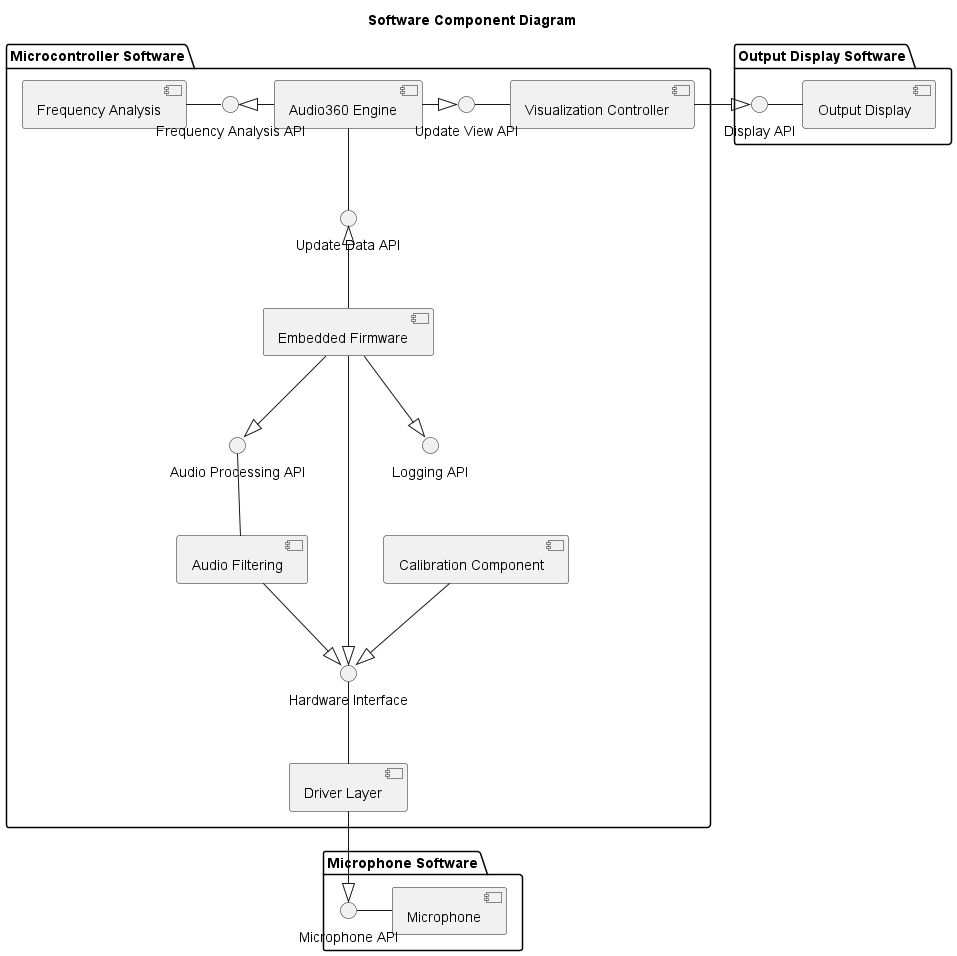
\includegraphics[width=0.9\textwidth]{diagrams/s1_component_diagram.png}
    \caption{Software component diagram.}
    \label{fig:software_component_diagram}
\end{figure}

\subsubsection{Software Components}

\begin{itemize}
  \item \textbf{Embedded Firmware:} \label{comp:embedded_firmware}
  Main component responsible for managing all embedded software on the
  Microcontroller.

  \item \textbf{Driver Layer:} \label{comp:driver_layer}
  Component responsible for providing drivers on the microcontroller. It
  provides interfaces for high level applications to interact with
  hardware components external to the microcontroller

  \item \textbf{Audio Filtering:} \label{comp:audio_filtering}
  Component responsible for processing raw audio signals in real-time sent
  by the microphones.

  \item \textbf{Calibration Component:} \label{comp:calibration}
  Component for calibrating hardware including microphones and output display.
  
  \item \textbf{Audio360 Engine:} \label{comp:audio360Engine}
  Main component responsible for running Audio360 features. It serves as the
  primary interface and controller for the Audio360 system. The component is
  designed to be hardware agnostic, allowing seamless integration with any
  firmware running on other hardware.
  
  \item \textbf{Frequency Analysis:} \label{comp:frequency_analysis}
  Component responsible for analyzing properties of processed frequency signals.
  Sub components of this includes audio classification and direction of arrival
  estimation.
  
  \item \textbf{Visualization Controller:} \label{comp:viz_controller}
  Component reposonsible for creating and sending visualization output to the
  \hyperref[comp:display]{output display}.
\end{itemize}

\subsubsection{Hardware Components}

\begin{itemize}
  \item \textbf{Microphone:}\label{comp:microphone}
  Component responsible for collecting audio signals from the environment.

  \item \textbf{Output display:}\label{comp:display} Component responsible for
  displaying visuals to the user.

  \item \textbf{Microcontroller:}
  \label{comp:microcontroller} Component responsible for executing the main
  software and interfacing with input and output peripheral devices.
\end{itemize}

\subsection{S.2 Functionality}

\subsubsection{\hyperref[comp:embedded_firmware]{Embedded Firmware}}
Functional Requirements
\begin{itemize}
  \item \label{FR1_1}\textbf{FR1.1:} The firmware shall schedule tasks
  based on its priority.
  
  \item \label{FR1_2}\textbf{FR1.2:} The firmware shall process and
  synchronize audio signals from all microphones connected to the
  microcontroller.

  \item \label{FR1_3}\textbf{FR1.3:} The firmware shall handle memory errors to
  prevent the micrcontroller from crashing.

  \item \label{FR1_4}\textbf{FR1.4:} The system shall perform continuous
  diagnostics on all hardware components to monitor hardware errors in
  real-time. This ensures the system can react to failures as soon as they 
  occur.
\end{itemize}

Non-Functional Requirements
\begin{itemize}
  \item \label{NFR1_1}\textbf{NFR1.1:} The firmware shall process audio
  signals in real-time with monotonic frame sequences. Earliest frames shall
  have higher priority.
  
  \item \label{NFR1_2}\textbf{NFR1.2:} The firmware shall operate
  faster than the connected microphone sample rate 44100 Hz, refering to
  \hyperref[NFR7_1]{NFR7.1}.
\end{itemize}

\subsubsection{\hyperref[comp:driver_layer]{Driver Layer}}
Functional Requirements
\begin{itemize}
  \item \label{FR2_1}\textbf{FR2.1:} The driver layer shall provide an
  interface for higher level software to interact with the hardware on the
  microcontroller.

  \item \label{FR2_2}\textbf{FR2.2:} The driver layer shall process 
  hardware interface requests based on system permissions of the requester.

  \item \label{FR2_3}\textbf{FR2.3:} The driver layer shall return error codes 
  upon return to higher-level software to support error handling.

  \item \label{FR2_4}\textbf{FR2.4:} The driver shall maintain data integrity
  on memory slots that is actively being used.
\end{itemize}

Non-Functional Requirements
\begin{itemize}
  \item \label{NFR2_1}\textbf{NFR2.1:} The driver shall immediately propagate
  any errors to the firmware layer for proper error handling.
\end{itemize}

\subsubsection{\hyperref[comp:audio_filtering]{Audio Filtering}} 
Functional Requirements
\begin{itemize}
  \item \label{FR3_1}\textbf{FR3.1:} The audio filtering component shall
  convert digital audio waveform to frequency domain.

  \item \label{FR3_2}\textbf{FR3.2:} The audio filtering component shall
  normalize the amplitude of incoming and outgoing signals.

  \item \label{FR3_3}\textbf{FR3.3:} The audio filtering component shall
  filter incoming audio signals to reduce frequency
  \hyperref[def:spectral_leakage]{spectral leakage}.

  \item \label{FR3_4}\textbf{FR3.4:} The audio filtering component shall
  use available hardware acceleration method for efficient computations.

  \item \label{FR3_5}\textbf{FR3.5:} The audio filtering component shall
  detect and flag audio anomalies such as clipping, lost signal and silence.
  This enables identification of microphone or signal path faults.
\end{itemize}

Non-Functional Requirements
\begin{itemize}
  \item \label{NFR3_1}\textbf{NFR3.1:} The audio filtering component shall 
  represent audio signals in the frequency domain with less than 10\% error from
  the true value.
  \item \label{NFR3_2}\textbf{NFR3.2:} The audio filtering component shall be
  scalable to handle different input signal sizes without missing timing
  constraints defined in \hyperref[NFR1_2]{NFR1.2} for input signal size up to
  4096 frames.

  \item \label{NFR3_3}\textbf{NFR3.3:} The audio filtering component shall have
  an audio processing success rate end to end of atleast 90\% over 60 seconds.
\end{itemize}

\subsubsection{\hyperref[comp:audio360Engine]{Audio360 Engine}} 
Functional Requirements
\begin{itemize}
  \item \label{FR4_1}\textbf{FR4.1:} The Audio360 Engine shall retrieve data,
  such as frequency domain and errors, from the microcontroller via the driver
  layer for further processing.

  \item \label{FR4_2}\textbf{FR4.2:} The Audio360 Engine shall notify dependent
  components when new frequency data is available. The latest data shall always
  be used.

  \item \label{FR4_3}\textbf{FR4.3:} The Audio360 Engine shall control the flow
  of processed audio data from audio frequency analysis to visualization.

  \item \label{FR4_4}\textbf{FR4.4:} The Audio360 Engine shall disable audio
  classification and directional analysis features until microphone faults
  addressed in \hyperref[FR3_5]{FR3.5} are resolved. This prevents the
  generation of unreliable or unsafe outputs.
\end{itemize}

Non-Functional Requirements
\begin{itemize}
  \item \label{NFR4_1}\textbf{NFR4.1:} The Audio360 Engine shall poll data
  without conflicting with ongoing microcontroller memory writes, ensuring no
  data loss.

  \item \label{NFR4_2}\textbf{NFR4.2:} The Audio360 Engine shall retrieve
  frequency data within the timing constraints of the embedded firmware defined
  in \hyperref[NFR1_2]{NFR1.2}.

  \item \label{NFR4_3}\textbf{NFR4.3:} The Audio360 Engine shall permanently
  discard microphone audio data immediately after completion of audio analysis.
\end{itemize}

\subsubsection{\hyperref[comp:frequency_analysis]{Frequency Analysis}} 
Functional Requirements
\begin{itemize}
  \item \label{FR5_1}\textbf{FR5.1:} The frequency analysis component shall
  classify sound sources based on features extracted from the frequency domain
  representation of the audio input signal.

   \item \label{FR5_2}\textbf{FR5.2:} The frequency analysis component shall
   estimate the direction of arrival of the audio source using frequency domain
   representation of the audio input signal. 
   
   \item \label{FR5_3}\textbf{FR5.3:} The frequency analysis component shall 
   represent the direction of arrival as an angle ($\theta$) in radians.
   $\theta$ is measured relative to the forward axis of the glasses frame
   to the sound source, Figure \ref{fig:coordinate_system}.

   \item \label{FR5_4}\textbf{FR5.4:} The frequency analysis component shall
   notify users when a sound classification result has low confidence or is
   unrecognized to prevent misleading contextual feedback.
\end{itemize}

\begin{figure}[H]     
    \centering 
    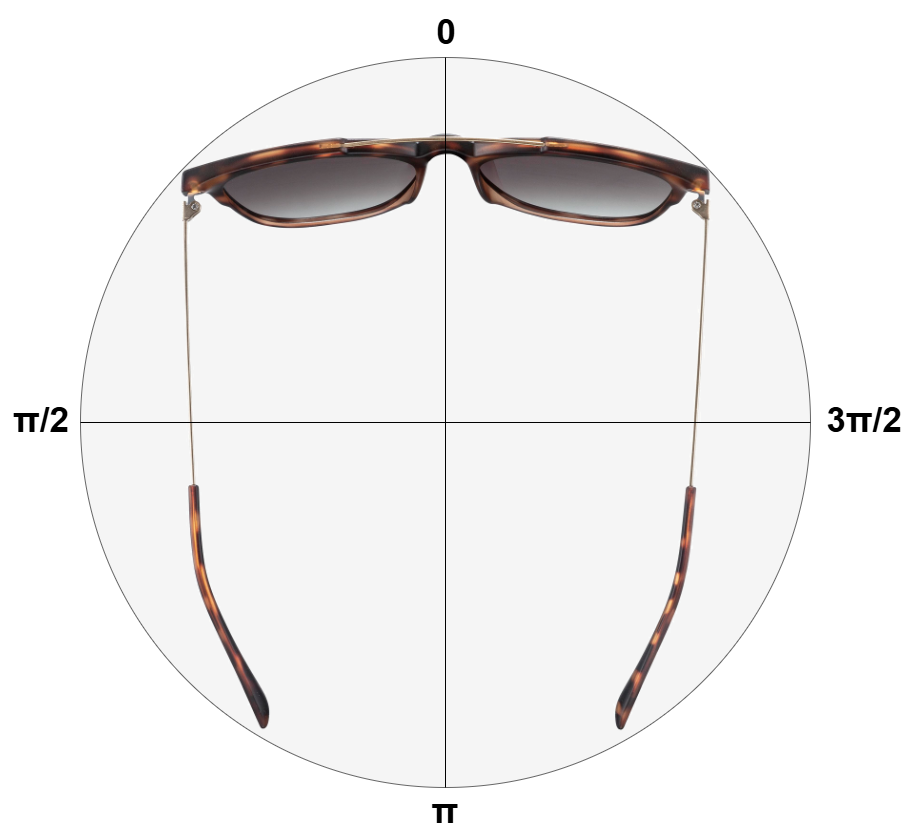
\includegraphics[width=0.75\textwidth]{diagrams/glasses_coordinate.png}
    \caption{Coordinate System.}
    \label{fig:coordinate_system}
\end{figure}

Non-Functional Requirements
\begin{itemize}
  \item \label{NFR5_1}\textbf{NFR5.1:} The frequency analysis shall classify
  atleast 3 distinct sound sources relevant to people who are hard of hearing.

  \item \label{NFR5_2}\textbf{NFR5.2:} The frequency analysis component shall
  achieve a minimum classification accuracy of 90\% under
  \hyperref[def:normal_operation_condition]{normal operating conditions}.

  \item \label{NFR5_3}\textbf{NFR5.3:} The component shall estimate the
  direction of arrival of an audio source with a maximum error of 45 degrees.
  This ensures reliable directional awareness for the user.
\end{itemize}

\subsubsection{\hyperref[comp:viz_controller]{Visualization Controller}}
Functional Requirements
\begin{itemize}
  \item \label{FR6_1}\textbf{FR6.1:} The visualization controller component
  shall notify users of the direction of an audio source whenever it is
  detected by the system.

  \item \label{FR6_2}\textbf{FR6.2:} The visualization controller component
  shall alert users when the core safety features such as direction
  determination or classification fail. This ensures that users are aware of
  degraded safety functions.
\end{itemize}

Non-Functional Requirements
\begin{itemize}
  \item \label{NFR6_1}\textbf{NFR6.1:} The visualization controller component
  shall prioritize to display the most safety-critical information at the
  time because display space is limited.
  \item \label{NFR6_2}\textbf{NFR6.2:} The visualization controller component
  shall present information in a non-intrusive manner, minimizing visual
  obstruction so users can safely perform external activities.
\end{itemize}

\subsubsection{\hyperref[comp:microphone]{Microphone}}
Functional Requirements
\begin{itemize}
  \item \label{FR7_1}\textbf{FR7.1:} The microphone shall collect soundwaves
  from its environment and translate to digital representation.

  \item \label{FR7_2}\textbf{FR7.2:} The microphone shall collect soundwaves
  with the human audiable range (20 Hz - 20 kHz) \cite{Neuroscience2001}.
\end{itemize}

Non-Functional Requirements
\begin{itemize}
  \item \label{NFR7_1}\textbf{NFR7.1:} The microphone shall collect soundwaves
  at 44100 Hz. According to Nyquist's theorem, audio sampling should be greater
  than two times the highest frequency to avoid aliasing \cite{DataForth2025}.
  The maximum frequecy audible to humans is approximately 20 kHz.
  \cite{Neuroscience2001}.
\end{itemize}

\subsubsection{\hyperref[comp:display]{Output Display}}
Functional Requirements
\begin{itemize}
  \item \label{FR8_1}\textbf{FR8.1:} The output display shall notify users of 
  the classified sound source.

  \item \label{FR8_2}\textbf{FR8.2:} The output display shall notify users of 
  the direction of the sound source.
\end{itemize}

Non-Functional Requirements
\begin{itemize}
  \item \label{NFR8_1}\textbf{NFR8.1:} The output display shall operate at a
  minimum of 30 display updates per second to ensure low latency and provide
  information to the user without perceptible delay.
\end{itemize}

\subsubsection{\hyperref[comp:microcontroller]{Microcontroller}}
Functional Requirements
\begin{itemize}
  \item \label{FR9_1}\textbf{FR9.1:} The microcontroller shall run the main
  \progname ~software in a closed environment. No external devices
  other than the microphones and output display shall be able to connect to it.
  This ensures protection against unauthorized access.
\end{itemize}

Non-Functional Requirements
\begin{itemize}
  \item \label{NFR9_1}\textbf{NFR9.1:} The microcontroller shall have a clock 
  speed of atleast 100 MHz to support audio sampling at 44100 Hz, derived
  from \hyperref[NFR7_1]{NFR7.1}.

  \item \label{FR9_2}\textbf{NFR9.2:} The microcontroller shall provide atleast
  four microphone inputs to support directional analysis of audio.
\end{itemize}


\subsection{S.3 Interfaces}
Audio360 is designed as a closed embedded system due to its safety-critical
application domain, refering to functional requirement \hyperref[FR9_1]{FR9.1}.
External access is intentionally restricted to ensure reliability, security,
and user safety.
The only user interface is the integrated visual display. The display provides
real-time information by notifying users of detected sounds and their
corresponding direction.
No external programmatic interfaces (APIs) will be provided. This design
decision ensures that system integrity is maintained and that no external
software can interfere with the safety-critical operation of the device.

\subsection{S.4 Detailed usage scenarios}
\wss{Examples of interaction between the environment (or human users) and the system: use cases, user stories.}

This section provides detailed versions of the high-level scenarios from \ref{item:G.5}, with specific technical details and interaction flows.

\subsubsection{S.4.1 Pedestrian Crossing Detection}
\textbf{User Story:} As a deaf individual, I want to be alerted when vehicles are approaching so I can cross streets safely.

\textbf{Scenario:} A user is walking in an urban environment and approaches a street intersection. As they prepare to cross, a car approaches from their left side.

\textbf{Interaction Flow:}
\begin{enumerate}
    \item System detects engine sound pattern characteristic of a vehicle
    \item DoA algorithm estimates direction
    \item Audio classification identifies the sound as a vehicle
    \item Smart glasses display visual indicator showing direction and notifies the user of a vehicle approaching
    \item User recognizes the alert and waits for the vehicle to pass before crossing safely
\end{enumerate}

\subsubsection{S.4.2 Kitchen Safety Alert}
\textbf{User Story:} As a deaf individual, I want to be notified of household safety sounds so I can respond to potential hazards.

\textbf{Scenario:} A user is cooking in their kitchen when a tea kettle on the stove begins to whistle.

\textbf{Interaction Flow:}
\begin{enumerate}
    \item Microphone array captures the high-pitched whistle sound
    \item System processes the audio and identifies the characteristic pattern
    \item DoA algorithm estimates the direction
    \item Audio classification identifies it as a kettle or alarm sound (90\% accuracy target)
    \item Smart glasses display directional indicator notifying the user of a kettle whistling ($\leq 1$s latency)
    \item User turns toward the alert and removes the kettle from heat, preventing potential hazard
\end{enumerate}

\subsubsection{S.4.3 Social Interaction}
\textbf{User Story:} As a deaf individual, I want to know when someone is trying to get my attention so I don't miss social interactions.

\textbf{Scenario:} A user is in a crowded room when someone calls their name from across the space.

\textbf{Interaction Flow:}
\begin{enumerate}
    \item System captures audio from all directions through the microphone array
    \item Voice activity detection identifies human speech patterns
    \item DoA algorithm estimates the direction
    \item Audio classification identifies the sound as speech or human voice
    \item Smart glasses display the information with directional arrow
    \item User turns in the indicated direction to make eye contact and engage in conversation
\end{enumerate}

\subsubsection{S.4.4 Workplace Awareness}
\textbf{User Story:} As a deaf worker, I want to be aware of industrial safety warnings so I can maintain workplace safety.

\textbf{Scenario:} A user is working in an industrial setting when a forklift begins reversing nearby, emitting a warning beep.

\textbf{Interaction Flow:}
\begin{enumerate}
    \item System detects the characteristic beeping pattern through microphone array
    \item DoA algorithm estimates the direction
    \item Audio classification identifies it as a warning signal or industrial alarm
    \item Smart glasses display prominent visual indicator notifying the user of a forklift backing up and directional arrow
    \item User steps aside to maintain a safe distance from the moving equipment
\end{enumerate}

\subsection{S.5 Prioritization}

This section classifies all system behaviors, interfaces, and scenarios by their degree of criticality to ensure proper development prioritization and resource allocation. Requirements are organized into three criticality levels: Critical, Important, and Desirable, with corresponding development stages.

\subsubsection{S.5.1 Critical Requirements (Stage 1 - Foundation)}

Critical requirements form the essential foundation of the system and must be
implemented first. These requirements are necessary for basic system operation
and safety. \\
\newline
Estimated deadline: December 9th, 2025 \\
\newline

\textbf{Core Hardware and Infrastructure:}
\begin{itemize}
    \item \hyperref[FR7_1]{FR7.1} - Microphone soundwave collection and digital conversion
    \item \hyperref[FR7_2]{FR7.2} - Human audible range coverage (20 Hz - 20 kHz)
    \item \hyperref[NFR7_1]{NFR7.1} - 44100 Hz sampling rate
    \item \hyperref[FR9_1]{FR9.1} - Closed microcontroller environment
    \item \hyperref[NFR9_1]{NFR9.1} - Minimum 100 MHz clock speed
    \item \hyperref[FR9_2]{FR9.2} - Four microphone inputs for directional analysis
\end{itemize}

\textbf{Sound Classification:}
\begin{itemize}
    \item \hyperref[FR5_1]{FR5.1} - Sound source classification
    \item \hyperref[NFR5_1]{NFR5.1} - Classification of 3+ distinct sound sources
    \item \hyperref[NFR5_2]{NFR5.2} - 90\% classification accuracy
\end{itemize}

\textbf{Basic Audio Processing:}
\begin{itemize}
    \item \hyperref[FR1_2]{FR1.2} - Audio signal processing and synchronization
    \item \hyperref[FR3_1]{FR3.1} - Digital to frequency domain conversion
    \item \hyperref[FR3_2]{FR3.2} - Signal amplitude normalization
    \item \hyperref[NFR3_1]{NFR3.1} - Frequency domain accuracy ($\le 10\%$ error)
    \item \hyperref[NFR1_2]{NFR1.2} - Processing faster than 44100 Hz sample rate
\end{itemize}

\textbf{Error Handling and Reliability:}
\begin{itemize}
    \item \hyperref[FR1_3]{FR1.3} - Memory error handling
    \item \hyperref[FR1_4]{FR1.4} - Continuous hardware diagnostics
    \item \hyperref[FR2_3]{FR2.3} - Driver error code returns
    \item \hyperref[NFR2_1]{NFR2.1} - Immediate error propagation
\end{itemize}

\textbf{Basic Display Functionality:}
\begin{itemize}
    \item \hyperref[FR8_1]{FR8.1} - Sound source classification display
    \item \hyperref[FR8_2]{FR8.2} - Sound direction display
    \item \hyperref[NFR8_1]{NFR8.1} - 30 display updates per second
\end{itemize}

\subsubsection{S.5.2 Important Requirements (Stage 2 - Core Features)}

Important requirements implement the primary functionality that delivers the
system's main value proposition. These build upon the critical foundation. \\
\newline
Estimated deadline: February 9th, 2026 \\
\newline

\textbf{Direction of Arrival (DoA) Analysis:}
\begin{itemize}
    \item \hyperref[FR5_2]{FR5.2} - Direction of arrival estimation
    \item \hyperref[FR5_3]{FR5.3} - Angular representation in radians
    \item \hyperref[NFR5_3]{NFR5.3} - Maximum 45 degrees DoA error
\end{itemize}

\textbf{Advanced Audio Processing:}
\begin{itemize}
    \item \hyperref[FR3_3]{FR3.3} - Spectral leakage filtering
    \item \hyperref[FR3_4]{FR3.4} - Hardware acceleration utilization
    \item \hyperref[FR3_5]{FR3.5} - Audio anomaly detection
    \item \hyperref[NFR3_2]{NFR3.2} - Scalability to 4096 frames
    \item \hyperref[NFR3_3]{NFR3.3} - 90\% processing success rate
\end{itemize}

\textbf{System Integration:}
\begin{itemize}
    \item \hyperref[FR2_1]{FR2.1} - Driver layer hardware interface
    \item \hyperref[FR2_2]{FR2.2} - Permission-based hardware access
    \item \hyperref[FR2_4]{FR2.4} - Data integrity maintenance
    \item \hyperref[FR4_1]{FR4.1} - Audio360 Engine data retrieval
    \item \hyperref[FR4_2]{FR4.2} - Component notification system
    \item \hyperref[FR4_3]{FR4.3} - Data flow control
\end{itemize}

\textbf{Visualization and User Interface:}
\begin{itemize}
    \item \hyperref[FR6_1]{FR6.1} - Direction notification display
    \item \hyperref[FR6_2]{FR6.2} - Safety feature failure alerts
    \item \hyperref[NFR6_1]{NFR6.1} - Safety-critical information prioritization
    \item \hyperref[NFR6_2]{NFR6.2} - Non-intrusive display design
\end{itemize}

\subsubsection{S.5.3 Desirable Requirements (Stage 3 - Enhancement)}

Desirable requirements enhance system performance and user experience but are
not essential for basic operation. \\
\newline
Estimated deadline: April 9th, 2026 \\
\newline

\textbf{Advanced System Features:}
\begin{itemize}
    \item \hyperref[FR1_1]{FR1.1} - Priority-based task scheduling
    \item \hyperref[NFR1_1]{NFR1.1} - Monotonic frame sequence processing
    \item \hyperref[FR4_4]{FR4.4} - Feature disabling during microphone faults
    \item \hyperref[FR5_4]{FR5.4} - Low confidence classification notifications
\end{itemize}

\textbf{Performance Optimization:}
\begin{itemize}
    \item \hyperref[NFR4_1]{NFR4.1} - Conflict-free data polling
    \item \hyperref[NFR4_2]{NFR4.2} - Timing constraint compliance
    \item \hyperref[NFR4_3]{NFR4.3} - Immediate data disposal after analysis
\end{itemize}

\subsubsection{S.5.4 Scenario Prioritization}

\textbf{Critical Scenarios (Stage 1):}
\begin{itemize}
    \item \hyperref[S.4.2]{S.4.2} - Kitchen Safety Alert (highest safety impact)
    \item \hyperref[S.4.4]{S.4.4} - Workplace Awareness (industrial safety)
\end{itemize}

\textbf{Important Scenarios (Stage 2):}
\begin{itemize}
    \item \hyperref[S.4.1]{S.4.1} - Pedestrian Crossing Detection (public safety)
    \item \hyperref[S.4.3]{S.4.3} - Social Interaction (quality of life)
\end{itemize}

\subsubsection{S.5.5 Development Priority Rationale}

The prioritization follows a safety-first approach:

\begin{enumerate}
    \item \textbf{Stage 1 (Critical):} Establishes reliable hardware foundation and basic audio processing capabilities. Focuses on system stability and error handling to prevent failures that could compromise user safety.
    
    \item \textbf{Stage 2 (Important):} Implements core DoA and classification features that deliver the primary value proposition. Kitchen and workplace safety scenarios are prioritized due to their immediate safety implications.
    
    \item \textbf{Stage 3 (Desirable):} Adds performance optimizations and advanced features that enhance user experience but are not essential for basic safety functionality.
\end{enumerate}

This staged approach ensures that the most safety-critical features are implemented first, providing immediate value to users while building toward a complete system. The prioritization also considers technical dependencies, with lower-level components (hardware, drivers) being implemented before higher-level features (classification, visualization).

\subsection{S.6 Verification and acceptance criteria}

This section specifies the conditions under which the implementation will be 
deemed satisfactory. The verification criteria are organized by the major 
functional areas of the system and are directly traceable to the goals 
defined in Section 1 and the functional/non-functional requirements defined 
in Section S.2.

\subsubsection{S.6.1 Audio capture verification}

Related to \hyperref[goal:audio_capture]{Goal 1}, \hyperref[FR1_2]{FR1.2}, 
\hyperref[FR7_1]{FR7.1}, \hyperref[FR7_2]{FR7.2}, and \hyperref[NFR7_1]{NFR7.1}.

\begin{itemize}
\item \textbf{VC-1.1 Synchronized sampling:} The system shall demonstrate that 
all four microphones in the array capture audio samples with temporal alignment 
within ±10 microseconds, verified through oscilloscope measurements or 
timestamp analysis of captured data.

\item \textbf{VC-1.2 Sampling rate:} The system shall maintain a minimum 
sampling rate of 44.1 kHz across all microphone channels, verified through 
analysis of captured audio buffer timestamps.

\item \textbf{VC-1.3 Continuous operation:} The system shall demonstrate 
continuous audio capture for at least 1 hour without buffer overruns, 
dropped samples, or system crashes, verified through stress testing and 
log file analysis.
\end{itemize}

\subsubsection{S.6.2 Direction of arrival (DoA) verification}

Related to \hyperref[goal:audio_direction_analysis]{Goal 2}, \hyperref[FR5_2]{FR5.2}, 
\hyperref[FR5_3]{FR5.3}, and \hyperref[NFR5_3]{NFR5.3}.

\begin{itemize}
\item \textbf{VC-2.1 Single source accuracy:} For a single sound source in 
a controlled environment, the system shall estimate the direction of arrival 
with an angular error of less than or equal to 45° in at least 90\% of 
test cases, verified 
through testing with known sound source positions at various angles (0°, 45°, 
90°, 135°, 180°, 225°, 270°, 315°) around the user.

\item \textbf{VC-2.2 Processing latency:} The DoA estimation algorithm shall 
complete processing and output a direction estimate within 500 milliseconds 
of sound detection, verified through timestamp logging of detection and 
output events.

\item \textbf{VC-2.4 Range coverage:} The system shall detect and provide 
directional estimates for sounds originating from any direction in the full 
360° horizontal plane around the user, verified through systematic testing 
at multiple angles.

\item \textbf{VC-2.5 Consistency:} For a stationary sound source, the system 
shall provide consistent direction estimates with a standard deviation of 
less than or equal to 45° over 10 consecutive measurements, 
verified through repeated testing.
\end{itemize}

\subsubsection{S.6.3 Sound classification verification}

Related to \hyperref[goal:audio_identification_analysis]{Goal 3}, 
\hyperref[FR5_1]{FR5.1}, \hyperref[FR5_4]{FR5.4}, 
\hyperref[NFR5_1]{NFR5.1}, and \hyperref[NFR5_2]{NFR5.2}.

\begin{itemize}
\item \textbf{VC-3.1 Classification accuracy:} The audio classification system 
shall achieve at least 90\% accuracy in identifying sound categories from a 
predefined set (including at minimum: speech, vehicle sounds, alarms, and 
household appliances), verified through testing with a labeled dataset of at 
least 100 sound samples across all categories.

\item \textbf{VC-3.2 Processing latency:} The classification algorithm shall 
complete processing and output a classification label within 1 second of 
sound detection, verified through timestamp logging.

\item \textbf{VC-3.3 Category coverage:} The system shall support 
classification of at least 5 distinct sound categories relevant to safety 
and daily life, verified through documentation of the classification model 
and testing with representative samples from each category.

\item \textbf{VC-3.4 Handling unknown sounds:} The system shall gracefully 
handle sounds that do not match any trained category by either assigning a 
low-confidence score or providing a generic label (e.g., ``unknown sound''), 
verified through testing with sounds outside the training set.
\end{itemize}

\subsubsection{S.6.4 Visual display verification}

Related to \hyperref[goal:visual_display]{Goal 4}, \hyperref[FR6_1]{FR6.1}, 
\hyperref[FR8_1]{FR8.1}, \hyperref[FR8_2]{FR8.2}, \hyperref[NFR6_2]{NFR6.2}, 
and \hyperref[NFR8_1]{NFR8.1}.

\begin{itemize}
\item \textbf{VC-4.1 Display latency:} The complete system pipeline from sound 
detection to visual display on the smart glasses shall complete within 1 
second (less than or equal to 1s end-to-end latency), verified through 
synchronized video recording of sound source activation and display appearance.

\item \textbf{VC-4.2 Display visibility:} Visual indicators on the smart 
glasses shall be clearly visible and distinguishable under typical indoor 
and outdoor lighting conditions, verified through user testing and subjective 
evaluation by at least 3 test participants.

\item \textbf{VC-4.3 Non-obstruction:} Visual indicators shall not obstruct 
more than 20\% of the user's field of view at any given time, verified 
through measurement of display area relative to total viewable area.
\end{itemize}

\subsubsection{S.6.5 User interaction verification}

Related to \hyperref[goal:user_friendly_interaction]{Goal 5}, 
\hyperref[FR6_2]{FR6.2}, and \hyperref[NFR6_1]{NFR6.1}.

\begin{itemize}
\item \textbf{VC-5.1 Setup simplicity:} A new user shall be able to power on 
the device and begin receiving audio alerts within 5 minutes without requiring 
external documentation, verified through timed user testing with participants 
unfamiliar with the system.

\item \textbf{VC-5.2 Calibration process:} If calibration is required, the 
process shall be completable within 2 minutes and require no
user actions, verified through testing.
\end{itemize}

\subsubsection{S.6.6 System reliability verification}

Related to \hyperref[FR1_3]{FR1.3}, \hyperref[FR1_4]{FR1.4}, \hyperref[FR2_3]{FR2.3}, 
\hyperref[FR3_5]{FR3.5}, \hyperref[FR4_4]{FR4.4}, \hyperref[NFR2_1]{NFR2.1}, 
\hyperref[NFR3_3]{NFR3.3}, and \hyperref[NFR4_1]{NFR4.1}.

\begin{itemize}
\item \textbf{VC-6.1 Startup reliability:} The system shall successfully 
complete initialization and enter operational mode in at least 95\% of power-on 
attempts, verified through repeated startup testing (minimum 20 trials).
\end{itemize}



\section{Project}

\subsection{P.1 Roles and personnel}\label{item: p1}

All project staff have responsibilities they must carry out in addition to the
 individual work required for deliverables. 
The roles, and qualifications for each assignment are outlined below. 

\begin{itemize}
  \item Leader (Sathurshan Arulmohan)
    \begin{itemize}
      \item \textit{Responsibilities:}
        \begin{itemize}
          \item Point of contact for professor and TAs. 
          \item Ensures that the team is on track to meet deadlines.
          \item Project planning and scheduling.
        \end{itemize}
      \item \textit{Qualifications:}
        \begin{itemize}
          \item Strong organizational and leadership skills. 
          \item Has experience in coordinating group projects and managing 
          timelines. 
          \item Strong communication skills. 
        \end{itemize}
    \end{itemize}
  \item Meeting Chair (Kalp Shah)
    \begin{itemize}
      \item \textit{Responsibilities:}
        \begin{itemize}
          \item Creates the agenda for meetings.
          \item Facilitates the meetings.
          \item Ensures that the team sticks to the agenda.
        \end{itemize}
      \item \textit{Qualifications:}
        \begin{itemize}
          \item Great time management and facilitation skills. 
          \item Strong interpersonal, communication and organizational skills. 
          \item Prior experience in leadering meetings. 
        \end{itemize}
    \end{itemize}
  \item Reviewer (Jay Sharma)
    \begin{itemize}
      \item \textit{Responsibilities:}
        \begin{itemize}
          \item Reviews all deliverables before deadline to ensure all sections
           are completed.
          \item Reach out to the reviewers of each section to ensure they 
          approve it before the deadline.
        \end{itemize}
      \item \textit{Qualifications:}
        \begin{itemize}
          \item Attention to detail and strong analytical skills.
          \item Experience in document quality assurance, and proof reading. 
          \item Understanding of project requirements and documentation 
          standards. 
        \end{itemize}
    \end{itemize}
  \item Note taker (Nirmal Chaudhari)
    \begin{itemize}
      \item \textit{Responsibilities:}
        \begin{itemize}
          \item Takes notes during meetings.
          \item Create meeting notes summary after the meeting ends to grasp 
          meeting content.
          \item Coordinates with project leader after meeting ends for action 
          items. 
        \end{itemize}
      \item \textit{Qualifications:}
        \begin{itemize}
          \item Strong written communication, and summarization skills. 
          \item Multi-tasking abilities, able to capture technical discussions 
          while contributiing to meetings. 
          \item Ability to type fast, with little error. 
        \end{itemize}
    \end{itemize}
  \item System Specialist (Omar Alam)
    \begin{itemize}
      \item \textit{Responsibilities:}
        \begin{itemize}
          \item Manages and validates system design at a high level. 
          \item Responsible for hardware \& software interfaces.
          \item Handles budgeting and expenses, ensures total budget remains 
          under \$500.
        \end{itemize}
      \item \textit{Qualifications:}
        \begin{itemize}
          \item Technical background in software and hardware system design. 
          \item Experience with system architecture and prototyping.  
          \item Basic knowledge of budgeting and resource allocation. 
        \end{itemize}
    \end{itemize}
\end{itemize}


Moreover, all project members share the following competencies as contributing 
members to the development of this project. 
\begin{itemize}
  \item Embedded software development.
  \item Strong software design for novel features. 
  \item Strong testing and debugging skills. 
\end{itemize}

In addition to responsibilities as developers on the team, each project member 
has been designated as an \textbf{expert} in a specific area of focus essential 
to the development of this system. 
The designated focus areas are outlined below:

\begin{itemize}
    \item Research in using hardware acceleration methods and other code 
    optimization methods for embedded development, since the system is
    deployed on microcontroller with limited CPU and memory space. 
    \textbf{(Sathurshan Arulmohan)}.
    \item Hardware integration, including implementation of low-level hardware
     interface for high-level software. 
    Features should be abstracted so that it can integrate with other hardware
     devices. Since the hardware requires an API integration
    for this, this focus area is needed. \textbf{(Omar Alam)}.
    \item Analysis of methods to extract directionality from a microphone array,
     since multple microphones needs to be processed.
    and run some algorithm to determine which direction it is coming from. This
     algorithm needs to be researched. \textbf{(Kalp Shah)}.
    \item Exploration of techniques for separating multiple audio sources from 
    a single microphone input using Independent Component Analysis (ICA).
    This focus area is required since the system's environment will contain a 
    mixture of sounds that need to analyzed and processed indepdently. 
    \textbf{(Jay Sharma)}.
    \item Development of audio-fingerprinting for classifying sound sources
    based on the frequency domain representation of the audio signal. This
    feature needs to comply with the processing and memory limits of the
    compute unit.\textbf{(Nirmal Chaudhari)}.
\end{itemize}

\noindent
All experts share the following responsibilities for their area of focus. 

\begin{itemize}
  \item Look through research articles, and technical evaluations to come up 
  with feasibile approaches for proposed methods. 
  \item Collaborate with other team members to discuss findings. 
  \item Maintain clear and organized documentation of sources and proposed 
  methods. 
  \item Complete implementation of the focus area in the system.
  \item Testing to validate and verify the feature.
\end{itemize}

\subsection{P.2 Imposed technical choices}

\textbf{Microcontroller:}  
The system shall use a dedicated microcontroller with a minimum clock speed of
100 MHz. This constraint is imposed to ensure that the audio processing tasks
defined in functional requirement \hyperref[NFR1_3]{NFR1.3} can be
completed within timing constraints. A microcontroller is also chosen
because it can be physically embedded within the glasses, ensuring
low power consumption, compact integration, and user comfort.

\textbf{Microphones:}  
The system shall use between two and four omnidirectional microphones to collect
audio data from the environment. This range of microphones enables directional
detection while minimizing hardware complexity, cost, and power consumption.

\textbf{Programming Languages:}  
The embedded firmware shall be implemented in C/C++. This choice is imposed
because compiled C/C++ binaries can be directly executed on any microcontroller,
and the language provides low level access to system resources, memory, and
hardware acceleration functions necessary for efficient audio processing.

\subsection{P.3 Schedule and milestones} \label{item: p3}   

To better understand the needs of the stakeholders, there are various milestones
 that need to be completed within the realm of the requirements process.
These milestones can be generalized as a list of tasks, with their deadlines 
outlined below.

\begin{enumerate}
  \item Initial Supervisor Consultation (2025-09-15) \label{item: p3-1}
  \item Extraction of project soft and hard goals (2025-09-22) 
  \label{item: p3-2}
  \item Technical analysis for feasibility of project goals (2025-09-29) 
  \label{item: p3-3}
  \item Extraction of requirements from goals and technical assessment 
  (2025-10-2) \label{item: p3-4}
  \item Requirements Documentation (2025-10-10) \label{item: p3-5}
  \item Validation Plan (2025-10-27) \label{item: p3-6}
  \item System Design Plan (2025-10-27) \label{item: p3-7}
  \item Verification \& Validation of system (2026-02-02) \label{item: p3-8}
  \item Consultation with primary stakeholder (TBD) \label{item: p3-9}
\end{enumerate}

\subsection{P.4 Tasks and deliverables}

\begin{enumerate}

  \item \textbf{Initial Supervisor Consultation (2025-09-15)}  

  \textbf{Tasks:}
  \begin{itemize}
      \item Meet with the supevisor to clarify the project vision. 
      \item Discuss key goals, available resources and expected POC outcomes. 
      \item Identify initial research domains. 
  \end{itemize}

  \textbf{Expected Outcomes:}
  \begin{itemize}
      \item Team has a shared understanding of project objectives and potential
       risks associated with the project scope and goals. 
      \item Defined list of research priorities outlined in section
      \hyperref[item: p1]{P.1}.
  \end{itemize}

  \vspace{0.8em}

  \item \textbf{Extraction of project soft and hard goals (2025-09-22)}  

  \textbf{Tasks:}
  \begin{itemize}
      \item Based on team elicitation, brainstorm and document list of soft 
      goals. 
      \item Deconstruct soft goals into a list of hard goals using definition,
       contribution, decomposition techniques. 
      \item Discuss trade-offs of defined hard goals. 
  \end{itemize}

  \textbf{Expected Outcomes:}
  \begin{itemize}
      \item Comprehensive list of soft and hard goals, clearly defining the 
      project direction. 
      \item Consensus among team members and supervisor on achievable project
       objectives. 
      \item Prioritized list of goals for verification testing. 
      \item Validated list of goals with primary stakeholders. 
  \end{itemize}

  \vspace{0.8em}

  \item \textbf{Technical analysis for feasibility of project goals 
  (2025-09-29)}  

  \textbf{Tasks:}
  \begin{itemize}
      \item Review research articles relevant to goals extracted during the 
      elicitation stage. 
      \item Conduct feasibility assessments for key goals set in the project. 
      \item Run small-scale prototype, or test to confirm technical viability. 
  \end{itemize}

  \textbf{Expected Outcomes:}
  \begin{itemize}
      \item Confirmation of which project goals are technically achievable 
      within the scope.
      \item Revised goals based on hardware and software capabilities. 
      \item Early identification of design constraints. 
  \end{itemize}

  \vspace{0.8em}

  \item \textbf{Extraction of requirements from goals and technical assessment 
  (2025-10-2)}

  \textbf{Tasks:}
  \begin{itemize}
      \item Translate validated soft and hard goals into specific system 
      requirements. 
      \item Identify dependencies and relationships between requirements. 
      \item Ensure each requirement is unambiguous, measurable and achievable 
      within the scope. 
  \end{itemize}

  \textbf{Expected Outcomes:}
  \begin{itemize}
      \item Drafted list of functional and non-functional requirements derived 
      from goals. 
      \item Clear mapping between project goals and corresponding requirements. 
  \end{itemize}

  \vspace{0.8em}

  \item \textbf{Requirements Documentation (2025-10-10)}  

  \textbf{Tasks:}
  \begin{itemize}
      \item Iteratively updating sections in SRS document based on the results 
      of different tasks mentioned in \hyperref[item: p3]{P.3}. 
  \end{itemize}

  \textbf{Expected Outcomes:}
  \begin{itemize}
      \item Completed Rev 0 SRS document
      \item Software architecture and design can commence with a clear path 
      using SRS as a guidance. 
  \end{itemize}

  \vspace{0.8em}

  \item \textbf{Validation Plan (2025-10-27)}  

  \textbf{Tasks:}
  \begin{itemize}
      \item Come up with a plan for validating the system meets the requirement 
      specification.
      This plan should be exhaustive enough to confirm that all of the
      stakeholders' goals have been met. 
  \end{itemize}

  \textbf{Expected Outcomes:}
  \begin{itemize}
      \item The V\&V deliverable has been completed, and clearly outlines the 
      plan for validation and verification. 
  \end{itemize}

  \vspace{0.8em}

  \item \textbf{System Design Plan (2025-10-27)}  

  \textbf{Tasks:}
  \begin{itemize}
      \item Each focus area expert works on completing the design plan for the 
      implementation of that feature. 
      \item The design plan will be communicated to the rest of the team and the
       project advisor for validation on the design
      and any feedback will be addressed. 
  \end{itemize}

  \textbf{Expected Outcomes:}
  \begin{itemize}
      \item Each focus area has a fully completed design plan based on the 
      investigation completed by the expert. 
      \item The plan has been written in Rev 0 of the Design Document
  \end{itemize}

  \vspace{0.8em}

  \item \textbf{Verification \& Validation of System (2026-02-02)}  

  \textbf{Tasks:}
  \begin{itemize}
      \item Using the Rev 0 V\&V report, team goes through plan for validation 
      and verification of the system against
      requirement specifications. 
      \item For any unmet requirements based on the validation plan, the team 
      re-assess the requirements to see it's priority 
      in the given timeline. Previous requirement documents are updated 
      accordingly. 
  \end{itemize}

  \textbf{Expected Outcomes:}
  \begin{itemize}
      \item All documentation has been updated based on the current 
      implementation of the system. 
      \item Team has a clear list of unmet requirements that need to be 
      addressed. 
  \end{itemize}

  \vspace{0.8em}
  
  \item \textbf{Consultation with primary stakeholder (TBD)}    

  \textbf{Tasks:}
  \begin{itemize}
      \item Meet with the McMaster Sign Language club to conduct a
      semi-structured interview.
      \item Document all findings from interview specific to the questions
      asked. 
      \item Update stakeholder goals and requirements based on the results of 
      the interview. 
  \end{itemize}

  \textbf{Expected Outcomes:}
  \begin{itemize}
      \item SRS document has been updated to be inline with McMaster Sign 
      Language club needs. 
  \end{itemize}

  \vspace{0.8em}

\end{enumerate}


\subsection{P.5 Required technology elements}

\textbf{Microphones:}
Capable of sampling audio at 44100 Hz in order to capture the full audible
spectrum without aliasing. This complies with non function requirement 
\hyperref[NFR7_1]{NFR7.1}.
  
\textbf{Analog to Digital Converter:}
An analog to digital converter is required between each of the microphone and
the microcontroller to convert analog signals into digital form suitable
for processing.
  
\textbf{Microcontroller:} 
The microcontroller shall have sufficient processing speed and I/O bandwidth to
synchronously acquire data from multiple microphones without delays or sampling
misalignment.

\textbf{Output Display:}
A visual display module to show audio classification and detection to
\hyperref[stakeholder:hardHearing]{users who are hard of hearing}.

\subsection{P.6 Risks and mitigation analysis}
\wss{Potential obstacles to meeting the schedule of P.4, and measures for adapting the plan if they do arise.}

\subsection{P.7 Requirements process and report}
The development of this project requires iterating over various stages of the
requirements process. These stages include:

\begin{enumerate}
    \item \textbf{Elicitation}
    \begin{enumerate}
        \item Conduct stakeholder interviews and surveys to gather users' needs.

        \item Review background documents and research articles describing how
        core features have been implemented in the past.

        \item Consult with the technical supervisor of this application
        (\hyperref[itm:domain-experts]{MVM}) to gain insight into what
        approaches can be used. 
    \end{enumerate}

    \item \textbf{Analysis}
    \begin{enumerate}
        \item Based on information retrieved from the elicitation process,
        derive a list of soft and hard goals for the application.

        \item Using the goals defined previously, derive a list of key
        requirements. This will be influenced by the goals of the stakeholders,
        but also input on potential limitations based on discussion with the
        supervisor.

        \item Group requirements into functional vs.\ non-functional categories.

        \item Prioritize requirements using the MoSCoW framework (Must, Should,
        Could, Won't).

        \item Iteratively evaluate defined requirements based on new constraints
        that arise during implementation. 
    \end{enumerate}

    \item \textbf{Documentation}
    \begin{enumerate}
        \item Write requirements in a structured format that is clear, testable,
        and unambiguous.

        \item Use labels for different requirements and goals for traceability. 
    \end{enumerate}

    \item \textbf{Specification}
    \begin{enumerate}
        \item Using the \texttt{docs/} folder in the main repository for this
        project, update the various reports with the latest information based on
        what was discussed or finalized in other stages of the elicitation
        process. 
    \end{enumerate}

    \item \textbf{Validation}
    \begin{enumerate}
        \item Share draft requirements with stakeholders for confirmation. 
        \item Share requirements with the project supervisor to get expert
        opinion on feasibility of requirements. 
        \item Within the team, ensure the requirements are feasible, measurable,
        and aligned with the project scope. 
    \end{enumerate}
\end{enumerate}


As this project follows the V-model methodology, Figure
\ref{fig:v-model-process}, the team will aim to make the various stages of the
requirements process mentioned above linear. Since although this model allows
the team to re-visit previous parts, it will cost a lot to change in later
stages of the project. This is why this team is heavily prioritizing the initial
stages of the requirements process. 

\begin{figure}[H]
    \centering
    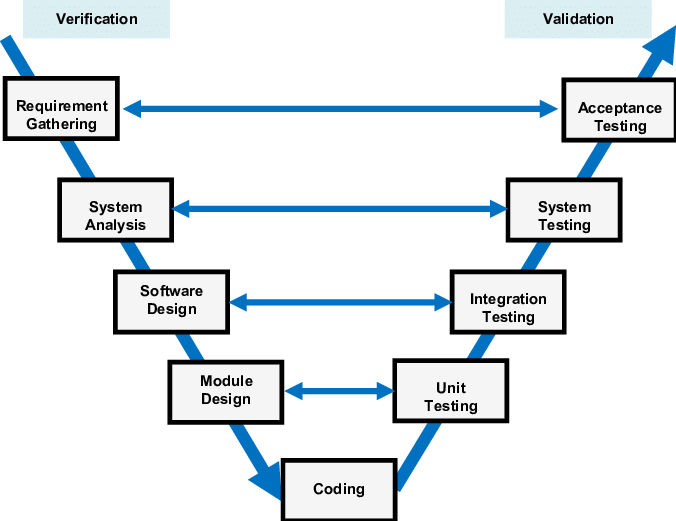
\includegraphics[width=0.75\textwidth]{./diagrams/v_model.png}
    \caption{Illustration of the v-model process.}
    \label{fig:v-model-process}
\end{figure}

\newpage
\bibliographystyle{IEEEtran}
\bibliography{../../refs/References}

\newpage
\section*{Appendix --- Reflection}

Questions 3 and 5 are answered as a team.

\begin{enumerate}
  \item What went well while writing this deliverable? 

  \textbf{Kalp:} I think what went really well during the writing of the SRS
  document was the frequent in-person work sessions. We were all able to sit
  together in a room, quickly review each other's work, make changes, discuss
  unclear assignments, and so on. This process, compared to the individual
  writeup and review process we used earlier, was much more efficient and
  effective, especially since this document was very interdependet (goals
  section for example having content related to the requirements section).
  
  \textbf{Nirmal Chaudhari:} Coming up with the schedule and milestone for this
  project was relatively easy for the elicitation and documentation stages since
  it was basically just a recap and coherent with what we just went through.
  Moreover, since our team had come up with the list of focus areas in advance,
  coming up with team roles and added responsibilities was relatively easy as
  well. 
  
  \textbf{Sathurshan:} In this deliverable, the team effectively collaborated on
  specific sections, allowing us to provide constructive feedback and
  iteratively refine our requirements during the initial write-up. This process
  helped align our goals for the system and provided a clearer understanding of
  what needed to be achieved.

  \textbf{Omar}: Throughout the deliverable writing process, the team
  communicated effectively and responded to feedback on the pull requests in a
  timely manner. This allowed us to rapidly iterate on the document. Since
  everyone brings an equal level of commitment and enthusiasm to the project, it
  made the collaboration process smooth and enjoyable.

  \textbf{Jay:} Building on our earlier deliverables made the writing process 
  much smoother. Having already defined the problem scope and development plan 
  gave us a solid foundation to work from, so translating those ideas into 
  detailed requirements felt natural. The structured template also helped keep 
  everything organized, making it easier to ensure completeness across all 
  sections. 

  \item What pain points did you experience during this deliverable, and how did
  you resolve them?

  \textbf{Kalp:} I think the main pain point was the way that we divided up the
  work on the document since many of the sections were dependent on each other.
  This often lead to some people on the team waiting for others to finish their
  section before they could start their own so that there wasn't conflicting
  information or text in the document. This process was slighly improved with
  the frequent in-person work sessions, but it was still a pain point.
  
  \textbf{Nirmal Chaudhari:} While working on the environment section, intially
  coming up with the list of components in the environment the system will have
  to interact with as difficult. This is because of the ambuguity that initially
  existed with what we can consider the "environment" for this system. This
  unclearity was resolved by coming up with a very high level use-case scenario
  of what a typical person would be interacting with when using the device.
  \textbf{Sathurshan:} Many sections were dependent on others being completed
  first, which blocked some of the writing process. With the granted extension,
  several sections were delayed, leading to a time crunch toward the end. To
  address this, the team organized multiple collaborative work sessions to work
  on the SRS document together. This allowed us to exchange ideas in real time,
  resolve blockers quickly, and progress in parallel. Moving forward, during the
  project planning stage, the team should prioritize dependency related issues
  and set internal deadlines to ensure smoother progress.

  \textbf{Omar}: There was some friction when it came to sections that relied on
  other sections being completed first. However, the team was able to work
  through these issues by holding several in-person and virtual meetings to
  discuss the document and make progress together. This allowed us to quickly
  resolve any blockers and ensure that everyone was on the same page.

  \textbf{Jay:} Striking the right balance between technical precision and 
  readability was challenging. Some sections needed enough detail to be 
  actionable, but too much made them hard to follow. We addressed this by 
  reviewing each other's sections and providing feedback on clarity, which 
  helped us converge on a consistent level of detail throughout the document. 

  \item How many of your requirements were inspired by speaking to your
  client(s) or their proxies (e.g. your peers, stakeholders, potential users)?

  A lot of the requirements related to focus areas defined in our SRS document
  were inspired by our project supervisor. He gave great insight into what major
  components need to be researched for this system to work. For example, he went
  over the requirement of needing 4 ADC converters in our microprocessor to
  retrieve synchronized audio input across all 4 microphones. If he didn't give
  this insight early on, the team would have been stuck in the later stages on
  the project with a microprocessor that will not work well for this system.
  Furthermore, he gave good information of how the team can go about using
  Independent Component Analysis to seperate audio into sources. He also
  mentioned we shouldn't use deep machine learning models for audio
  classification, since they won't be able to run on the microprocessor well. 

  
  \item Which of the courses you have taken, or are currently taking, will help
  your team to be successful with your capstone project.

  \textbf{Nirmal Chaudhari: } For this project the three courses I think will
  enable us to be the most successful are: Signals \& Systems, Requirements
  Engineering and Software Design 2. Signals \& Systems was important since the
  entire project revolves around processing and analyzing audio signals in the
  frequency domain. Requirements Engineering is important in helping us figure
  out our requirements and ensuring throughout the entire process that what we
  are building is the right thing. And Software Design 2 is useful in helping us
  implement best practices into the project, thus making it sustainable in the
  future.

  \textbf{Sathurshan:} 3MX3: signal processing, 2GA3: computer hardware
  architecture. 3RA3: software requirements, 2DA4: software design, 3A04:
  software architecture, 3S03: software testing.

  \textbf{Omar}: The courses that will help us the most with this project are:
  Signals and Systems (3MX3) - This course provides a solid foundation in signal
  processing, which is crucial for our project focused on audio signal analysis.
  Concurrent Programming (3BB4) - This course teaches us the core principles of
  concurrent programming which will be essential for implementing real-time
  processing on our microcontroller.

  \textbf{Kalp:} The courses that will probably help us the most for this
  project are 3MX3 (Signals \& Systems with Dr. Mohrenschildt). This course
  taught us many of the signal processing algorithms for that we will likely
  need to apply during our audio analysis for the system. Another good course
  would be 3A04 (Software Architecture) that taught us how to design and
  implement large scale software systems which will be important for our project
  as we we will be designing many modular components that work together. The
  planning techniques from the course, specifically, will be very useful.

  \textbf{Jay:} 3MX3 (Signals \& Systems) is definitely critical for 
  understanding audio processing and frequency analysis. Beyond that, 
  3BB4 (Concurrent Systems) will be valuable for managing real-time 
  constraints on the microcontroller, and 2GA3 (Computer Architecture) 
  will help us optimize performance on embedded hardware. The software 
  engineering courses like 3RA3 and 3S03 are also important for ensuring 
  we build a reliable, well-tested system.

  \item What knowledge and skills will the team collectively need to acquire to
  successfully complete this capstone project?  Examples of possible knowledge
  to acquire include domain specific knowledge from the domain of your
  application, or software engineering knowledge, mechatronics knowledge or
  computer science knowledge.  Skills may be related to technology, or writing,
  or presentation, or team management, etc.  You should look to identify at
  least one item for each team member.

  Each memmber of the team requires the following qualfiications as contributing
  developers to the team.

  \begin{itemize}
    \item Embedded software development.
    \item Strong software design for features being implemented on any
    microcontroller platform. 
    \item Strong testing skills.
    \item Strong debugging skills. 
  \end{itemize}

  In addition to this, since each team member is a focus area expert, they
  require the following skills and competencies to carry out that role.

  \begin{itemize}\setlength\itemsep{4pt}\setlength{\leftmargini}{2em}
    \item Look through research articles, and technical evaluations to come up
    with feasibile approaches for proposed methods. 
    \item Collaborate with other team members to discuss findings. 
    \item Maintain clear and organized documentation of sources and proposed
    methods. 
    \item Ensure that all research and implementation choices align with project
     objectives, timeline and budgeting costs. 
    \item Based on the confirmed approach, complete the full implementation of
    that focus in the system. 
    \item After implementation, create test cases that cover's the main
    functionality of the feature in that focus area. 
    \item Configure github pipeline to run those tests on every PR and merge
    into a feature branch. 
  \end{itemize}


  \item For each of the knowledge areas and skills identified in the previous
  question, what are at least two approaches to acquiring the knowledge or
  mastering the skill?  Of the identified approaches, which will each team
  member pursue, and why did they make this choice?

  \textbf{Kalp:} I think the main focus for knowledge areas to explore has to be
  around embedded software development and hardware integration. Since I've only
  done software development in industry before, I have experience developing, 
  testing, and debugging software, but have never explored the hardware side of
  the systems. 

  \textbf{Nirmal Chaudhari:} For embedded software development and strong
  software design, two approaches are available: (1) reviewing processor
  documentation and (2) practicing and test building small programs on the board
  to see how it targets key peripherals work. I will focus on the second
  approach since practical experience seems more important. For testing and
  debugging skills, the team can (1) study or use existing knowledge of
  frameworks and (2), conduct peer reviews with other members on the team. For
  this I would prefer the second approach since working with the team on real
  bugs would help me grow as a developer to see how others resolve bugs. For
  research and technical evaluation, the knowledge can be gained by (1) reading
  research papers existing in the focus area and (2) contacting domain experts
  like mvm for insights. I plan to start with the first option, since academic
  resources provides structure that can be referenced to later on.
 
  \textbf{Sathurshan:} I plan to focus on gaining knowledge in embedded software
  development, as it is something I want to specialize in the next few years.

  \textbf{Omar}: I believe the best way to learn any skill is by doing it and
  struggling through problems. Each microcontroller platform has its own quirks
  and tools. I plan to gain practical experience by developing smaller projects
  on the STM32 platform, which will help me understand its architecture. Each
  problem in our project can be subdivided into smaller projects, which will
  help me learn as I go. Additionally, I will refer to the STM32 documentation
  and online tutorials to supplement my learning.

  \textbf{Jay:} I'll be focusing on Independent Component Analysis (ICA) for 
  audio source separation. Two main approaches are: (1) implementing ICA 
  algorithms from research papers and testing them with sample audio data, 
  and (2) prototyping directly on the hardware with real microphone input. 
  I'll start with the first approach since it lets me validate the core 
  algorithms quickly without hardware dependencies, then transition to 
  hardware testing once we have a stable foundation. I'll also lean on our 
  supervisor's expertise to guide algorithm selection and avoid overly 
  complex solutions.

\end{enumerate}


\end{document}